\newif\ifmbeformat
\mbeformatfalse

\ifmbeformat
	\documentclass[nogrid]{MBE}%
\else
	\documentclass[twocolumn]{article}
	\usepackage{geometry}
	\newgeometry{
		top=1in,
		bottom=1in,
		outer=1in,
		inner=1in,
	}
	\usepackage{natbib}
	\renewcommand{\baselinestretch}{1.25}		
	\usepackage{authblk}
\fi

\usepackage[normalem]{ulem}
\usepackage{xcolor} 
\newcommand{\revch}[1]{{\color{blue} #1}}
\newcommand{\revcom}[1]{{\color{orange} #1}}
\newcommand{\revrem}[1]{{\color{red} \sout{#1}}}

\usepackage{url}
\usepackage{cuted}
\usepackage{amsmath}
\usepackage{subfig}
%\usepackage{caption}
\usepackage{tabularx}
\usepackage{longtable}
\usepackage{caption}
\usepackage{verbatim}
\usepackage{lipsum}
\usepackage{enumerate}
\usepackage{enumitem}
%load any additional packages
\usepackage{amssymb}
\usepackage{scalerel,stackengine}
\stackMath
\newcommand\reallywidehat[1]{%
	\savestack{\tmpbox}{\stretchto{%
			\scaleto{%
				\scalerel*[\widthof{\ensuremath{#1}}]{\kern-.6pt\bigwedge\kern-.6pt}%
				{\rule[-\textheight/2]{1ex}{\textheight}}%WIDTH-LIMITED BIG WEDGE
			}{\textheight}% 
		}{0.5ex}}%
	\stackon[1pt]{#1}{\tmpbox}%
}
\usepackage{amsfonts}
\usepackage{mathtools}
\usepackage{multirow}
\usepackage{bibentry}
%\usepackage{epstopdf} 
%\usepackage{xr}
%\usepackage[landscape,a4paper]{geometry}
\usepackage{booktabs} 
\usepackage{colortbl} 
%\usepackage{xcolor} 
%\usepackage{xfrac}
%\newcommand{ra}[1]{renewcommand{arraystretch}{#1}}
%\usepackage{pdflscape}
%\usepackage{longtable}
%\usepackage{stackrel}
\usepackage{hyperref}
%\usepackage{graphicx}
%\usepackage{svg}
\usepackage{setspace}
%\usepackage{refcheck}
%\usepackage{listings}
%\usepackage{color} 
\usepackage{array}
\usepackage{xr}
\externaldocument[supplementary-]{supplementary}


\newif\iffigures
\figurestrue

\ifmbeformat
\jshort{mst}

\volname{}

\jvolume{0}

\jvol{}

\jissue{0}

\pubyear{2013}

\mstype{Article}

\artid{012}

\access{Advance Access publication March 3, 2013}
\fi

\newcommand{\abstractext}{We present a probabilistic model of protein evolution that captures several important features of protein sequence and local structure. The key feature being  dependencies between neighbouring amino acid positions that are temporal in nature due to sequence mutations that occur during evolution. The model is trained on a large number of protein alignments and corresponding phylogenetic trees that represent the evolutionary history of the aligned proteins. This yields a model that acts as a rich prior distribution over protein evolution that can be used to perform several important inference tasks. One such task being Bayesian reconstruction of ancestral virus protein sequences, which we demonstrate to have better accuracy than competing methods. The model provides a complete probabilistic description of each protein's backbone structure using an angle and bond length representation. Structure evolution is modelled jointly with sequence, permitting ancestral structures and sequences to be reconstructed in a phylogenetically rigorous manner. Likewise, the model can perform homology modelling to predict the unknown local backbone structure of a known protein sequence using additional information from potentially large numbers of homologous proteins.  The model is highly flexible with respect to input, implying that arbitrary combinations of protein sequences and structures can be used when performing various inference tasks. The current model does not capture global features of protein structure that are necessary for accurate homology modelling or reconstruction of ancestral three-dimensional structures. However, it is ultimately expected to be combined with protein structure prediction models that account for such long-range dependencies, but that do not account for evolutionary information that can substantially enhance predictions of structures.}

\begin{document}

\title{Reconstructing ancestral protein	sequences and structures}

\ifmbeformat
\author[Golden et al.]{Michael \surname{Golden},$^{\ast,1}$, Jotun Hein,$^{2}$ Thomas Hamerlyck,$^{3}$ and Oliver Pybus,$^{1}$}

\address{
$^{1}$Department of Zoology, University of Oxford, UK\\
$^{2}$Department of Statistics, University of Oxford, UK\\
$^{3}$Bioinformatics Centre, Section for Computational and RNA Biology, Department of Biology and Image Section, Department of Computer Science, University of Copenhagen\\
}

\history{Received 13 July 2017; reviews returned 26 November 2017; accepted 30 November 2017}

\coresp{E-mail: golden@phylo.dev}

%\datade{Protein families were obtained from the HOMSTRAD database.}

\editor{Name Surname}

\else
\author[1]{Michael Golden}
\author[2]{Thomas Hamelryck}
\author[1]{Oliver Pybus}
\affil[1]{Department of Zoology, University of Oxford, UK}
%\affil[2]{Department of Statistics, University of Oxford, UK}
\affil[2]{Bioinformatics Centre, Section for Computational and RNA Biology, Department of Biology and Image Section, Department of Computer Science, University of Copenhagen}
\fi


\ifmbeformat
\abstract{\abstractext}
\keyword{Evolution, protein structure, probabilistic model}
\maketitle

\else

\onecolumn
\maketitle
\begin{abstract}
\normalsize
\abstractext
\end{abstract}
\twocolumn
\fi



\section{Introduction}

%%% Methods %%%
\section{Methods}

\subsection{Model}
\begin{figure*}
	\centering
	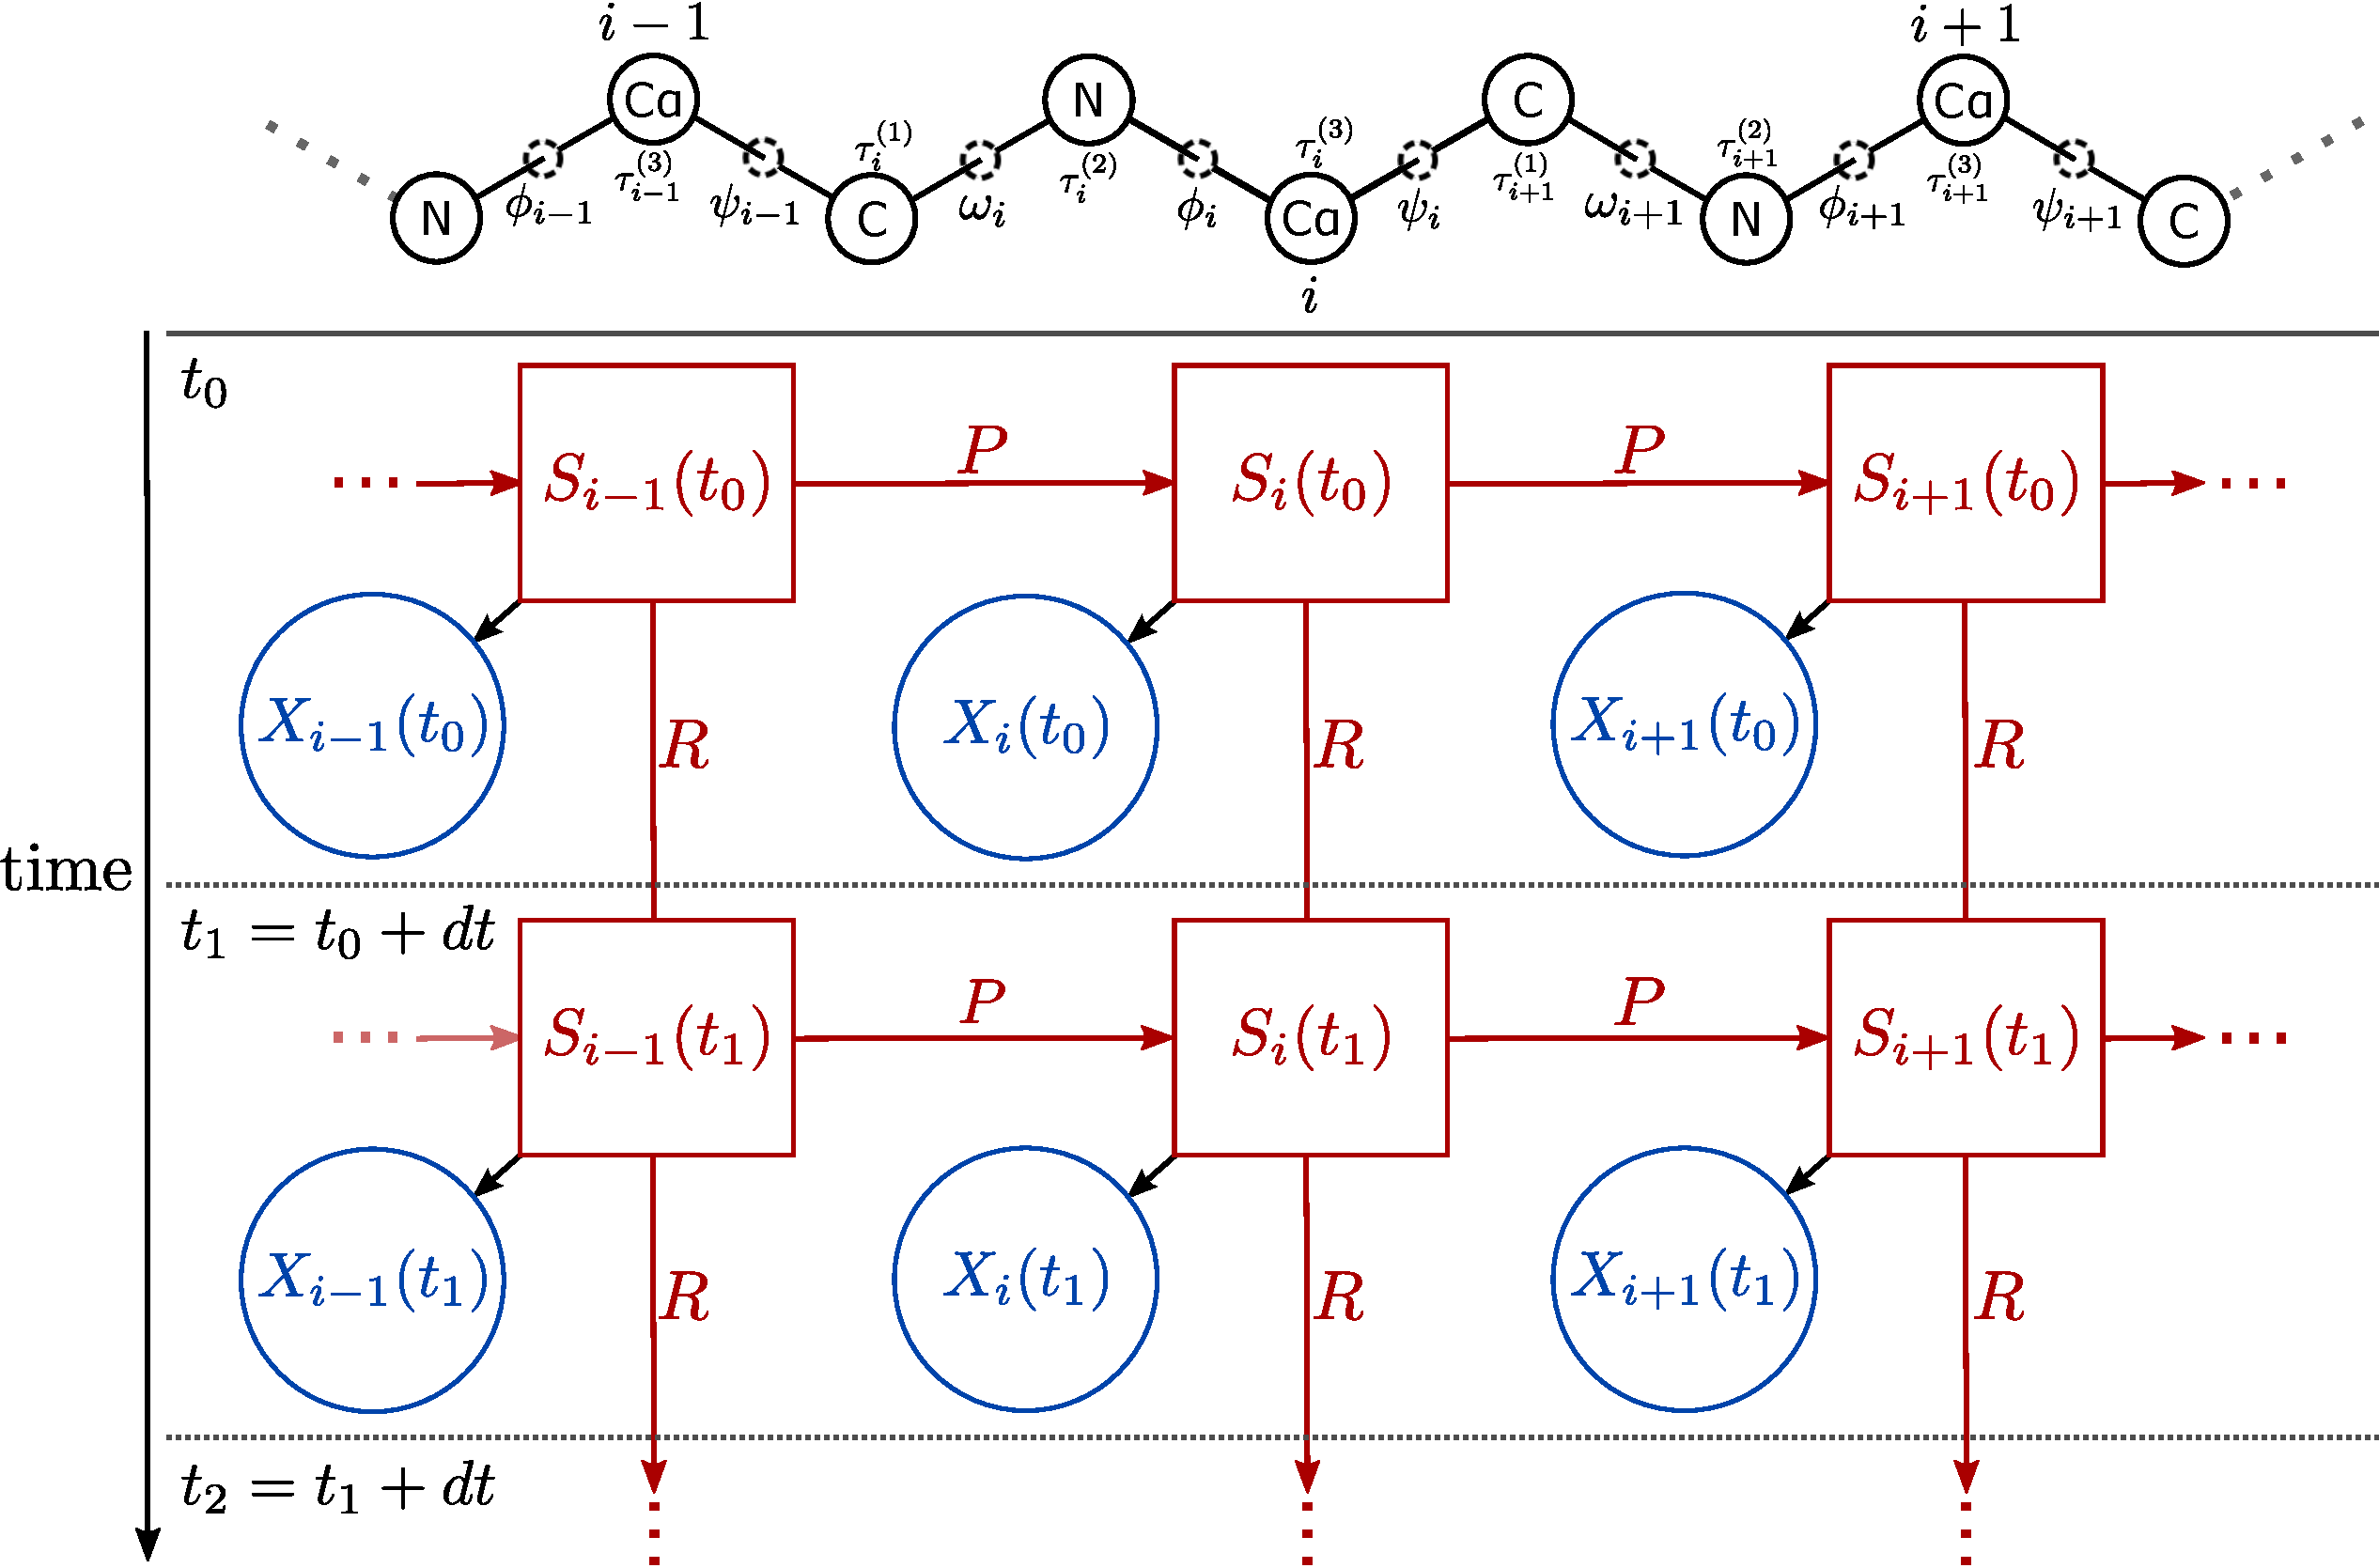
\includegraphics[width=1.75\columnwidth]{figures/model-structure-alt-final.pdf}
	\caption{Above: a depiction of a protein backbone (three amino acids long) with the $\omega$, $\phi$ and $\psi$ dihedral angles and the three additional bond angles ($\tau^{(1)}_{i}$, $\tau^{(2)}_{i}$, $\tau^{(3)}_{i}$) shown. Bond lengths are implicit. Bond angles and bond lengths are not to scale. Also shown are $\text{C}_{\alpha}$ atoms which attach to the amino acid side-chains. Each amino acid side-chain determines the characteristic nature of each amino acid. Every amino acid position corresponds to a hidden node in the model below.\newline
	Below: Graphical depiction of the model architecture showing three amino acid positions ($i-1$, $i$, and $i+1$) at two time instants ($t_0$ and $t_1$) along a single branch of a phylogenetic tree. Note that $S_{i}(t)=\big(H_{i}(t),A_{i}(t)\big)$.}%
	\label{fig:model-structure}%
\end{figure*}

\subsubsection{Model of a single protein}
A single protein consisting of $n$ amino acids:
\begin{align*}
 P_a  & = (H_a, A_a, X_a)\\
 & =\langle (H^{1}_a, A^{1}_a,X^{1}_a),\ldots,(H^{n}_a, A^{n}_a,X^{n}_a) \rangle
\end{align*}
is a sequence of aligned sites where each site $i$ is associated with a discrete-valued hidden state, $H_a^{i}$ (taking on one of $h$ possible values), a discrete-valued amino acid observation, $A_a^{i}$ (representing one of the twenty possible amino acids), and a corresponding vector of continuous-valued structural observations $X_a^{i}$ representing the backbone structure of the protein.

\paragraph{Structural observations}
The set of structural observations, $X_a^{i}$, at a particular site, $i$, consists of nine continuous-valued variables: three dihedral angles ($\phi_{i},\psi_{i},\omega_{i}$), three additional bond angles ($\tau^{(1)}_{i}=\reallywidehat{C{\alpha}_{i-1},C_{i-1},N_{i}}$, $\tau^{(2)}_{i}=\reallywidehat{C_{i-1},N_{i},C{\alpha}_{i}}$, $\tau^{(3)}_{i}=\reallywidehat{N_{i},C{\alpha}_{i},C_{i}}$), and three bond lengths ($b_{i}^{(1)}=\overrightarrow{C_{i-1},N_{i}}$, $b_{i}^{(2)}=\overrightarrow{N_{i},C{\alpha}_{i}}$, $b_{i}^{(3)}=\overrightarrow{C{\alpha}_{i},C_{i}}$). 

Note that $\phi_{1}$, $\tau^{(1)}_{1}$, and $\tau^{(2)}_{1}$, are undefined at the first position in the peptide backbone of an unaligned protein. Similarly, $\psi_{n}$ and  $\omega_{n}$ are undefined for the last position, $n$, in each unaligned protein.

Given the structural observations, $X_{a}$, it is possible to exactly reconstruct the three-dimensional coordinates of each atom in a protein's backbone \citep{Parsons2005}.

The $\omega_{i}$ dihedral angle (which determines the cis/trans conformation) at each site $i$ is assumed to be distributed according a univariate von Mises (vM) distribution with mean $\mu_{\omega}$ and concentration parameter $\kappa_{\omega}$ conditional on the hidden state $H_{a}^{i}$ and the amino acid $A_{a}^{i}$:
\begin{equation}
\label{eq:omega_dist}
\begin{array}{ccc}
\omega_{i} & \sim & \text{vM}\big(\mu_{\omega}(H_{a}^{i},A_{a}^{i}),\,\ensuremath{\kappa_{\omega}(H_{a}^{i},A_{a}^{i})}\big).
\end{array}
\end{equation}

The $\phi_{i}$ and $\psi_{i}$ dihedral angles are assumed to be drawn from a bivariate von Mises (bvM) distribution with mean vector $\mu_{\phi,\psi}=\langle \mu_{\phi},\mu_{\psi} \rangle$ and covariance parameters $\kappa_{\phi,\psi}=\langle \kappa_{1},\kappa_{2},\kappa_{3} \rangle$:
\begin{equation}
\label{eq:phipsi_dist}
\begin{array}{ccc}
(\phi_{i},\psi_{i}) & \sim & \text{bvM}\big(\mu_{\phi,\psi}(H_{a}^{i},A_{a}^{i}),\,\ensuremath{\kappa_{\phi,\psi}(H_{a}^{i},A_{a}^{i})}\big),
\end{array}
\end{equation}
where $\kappa_{1}$ is the variance associated with $\phi$, $\kappa_{2}$ is the variance associated with $\psi$, and $\kappa_{3}$ is the correlation between $\phi$ and $\psi$,

The three additional bond angles ($\tau^{(1)}_{i}$, $\tau^{(2)}_{i}$, $\tau^{(3)}_{i}$) are each distributed according a univariate (vM) distribution conditional on the hidden state $H_{a}^{i}$ only:
\begin{equation}
\label{eq:angle_density}
\begin{array}{ccc}
\tau^{(1)}_{i} & \sim & \text{vM}\big(\mu_{\tau^{(1)}}(H_{a}^{i}),\,\ensuremath{\kappa_{\tau^{(1)}}(H_{a}^{i})}\big)
\\
\tau^{(2)}_{i} & \sim & \text{vM}\big(\mu_{\tau^{(2)}}(H_{a}^{i}),\,\ensuremath{\kappa_{\tau^{(2)}}(H_{a}^{i})}\big)
\\
\tau^{(3)}_{i} & \sim & \text{vM}\big(\mu_{\tau^{(3)}}(H_{a}^{i}),\,\ensuremath{\kappa_{\tau^{(3)}}(H_{a}^{i})}\big).
\end{array}
\end{equation}

The three bond lengths ($b_{i}^{(1)}>0$, $b_{i}^{(2)}>0$, $b_{i}^{(3)}>0$) are 
distributed according a truncated Multivariate Normal (MVN)
with mean vector, $\mathbf{\mu}$, of length 3 and a $3 \times 3$ covariance matrix, $\Sigma$, conditional on the hidden state $H_{a}^{i}$:
\begin{equation}
\label{eq:bond_density}
(b_{i}^{(1)}, b_{i}^{(2)}, b_{i}^{(3)})  \sim \text{MVN}\big(\mu(H_a^{i}),\,\Sigma(H_a^{i})\big).
\end{equation}
Note that the parameters in \eqref{eq:angle_density} and \eqref{eq:bond_density} are no longer conditional upon the amino acid observations $A_{a}^{i}$. This was done to reduce the number of model parameters, as the values of the three bond angles and three bond lengths are all largely invariant, implying that the values can be reasonably fixed. Despite this, we still opted to treat them as random variables so that the model gives a complete probabilistic description of a protein backbone structure.

\paragraph{Site likelihood}
The likelihood of a structural observation, $p\big(X_{a}^{i}\,|\,H_{a}^{i},A_{a}^{i},\hat{\theta}\big)$, at site $i$ conditional on the hidden state, $H^{i}_a$, and amino acid, $S^{i}_a$, is given by a product of the densities in Equations~\ref{eq:omega_dist}, \ref{eq:phipsi_dist}, \ref{eq:angle_density}, and \ref{eq:bond_density}.

\begin{figure*}
	\centering
	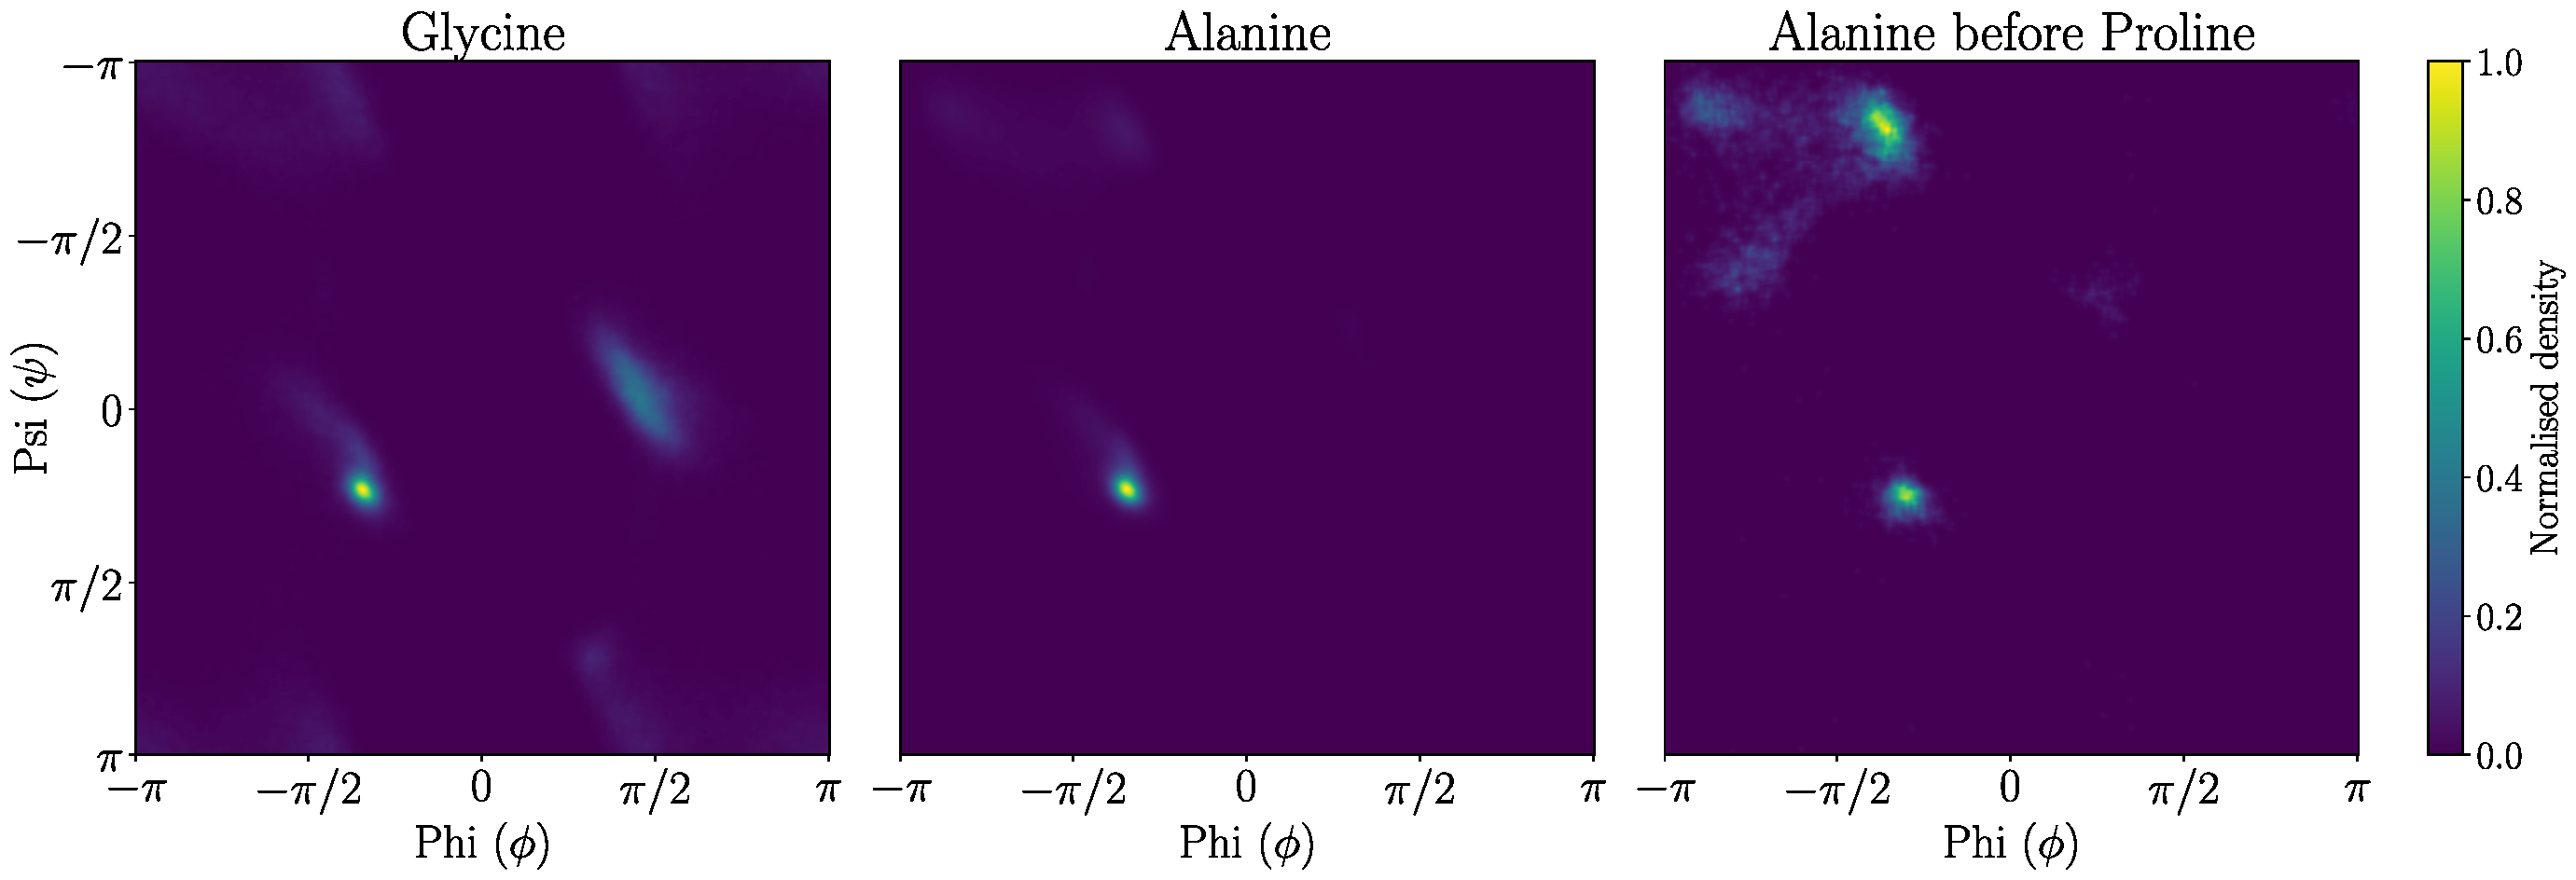
\includegraphics[width=2.0\columnwidth]{figures/ramachandran_empirical.pdf}
	\caption{Ramachandran plots depicting empirical distributions of $\phi$ and $\psi$ angle combinations under three different amino acid contexts. Glycine has the smallest amino acid side-chain and is therefore the least constrained. Alanine has a larger side-chain than glycine, constraining most $\phi$ and $\psi$ angle to lie near a single peak. When alanine precedes proline in the peptide backbone, the $\phi$ and $\psi$ angle combinations previously favoured become sterically hindered \revcom{MG: is this the correct terminology?}, favouring angle combinations at multiple peaks.}%
	\label{fig:ramachandranempirical}%
\end{figure*}

\paragraph{Hidden Markov model}
A sequence of structural observations representing a single protein backbone structure is modelled using a Hidden Markov Model (HMM). Hidden states in the HMM are primarily intended encode the angle and bond lengths distributions and their association with the different amino acids as specified in Equations~\ref{eq:omega_dist}-\ref{eq:bond_density}. However, the HMM is also critically to capture neighbouring dependencies, such as steric effects on dihedral angle conformations (Figure~\ref{fig:ramachandranempirical}). These neighbouring dependencies are captured using a $h\times{h}$ transition probability matrix  $P=p(H_{a}^{i}\,|\,H_{a}^{i-1},\hat{\theta})$.

We let $\Pi(a)$ denote the joint likelihood of a sequence of hidden states ($H_a$) and structural observations ($X_a$) conditional on a sequence of amino acids ($A_a$)  defined as follows:
\begin{align}
\label{eq:proteinlikelihood}
\Pi(a) = p(H_{a},A_{a},X_{a}\,|\,\hat{\theta}) = \notag \\
 p\big(A_{a}^{1},X_{a}^{1}\,|\,H_{a}^{1},\hat{\theta}\big)p(H_{a}^{1}\,|\,\hat{\theta})\notag \\
\times \prod_{i=2}^n p\big(A_{a}^{i},X_{a}^{i}\,|\,H_{a}^{i},\hat{\theta}\big)p(H_{a}^{i}\,|\,H_{a}^{i-1},\hat{\theta}),
\end{align}
where $p(H_{a}^{1}\,|\,\hat{\theta})$ is the initial probability of starting in state $H_{a}^{1}$ at the first site. Whilst  $\Pi(a)$ describes a single protein, it is used in the next section to `weight' an evolutionary model such that protein evolutionary trajectories are visited with probability proportional to $\Pi\times{\pi}$, where $\pi$ is weighting corresponding to the amino acid sequences.
\begin{comment}
The probability, $\Pi(a)$, of a set structural observations, $X_a$ conditioned on the corresponding hiddem state sequence, $H_a$,  the amino acid sequence, $S_a$, and model parameters, $\hat{\theta}$, is given by:
\begin{align}
\Pi(a) = p(X_{a}\,|\,H_{a},S_{a},\hat{\theta}) = \notag \\
\frac{1}{Z} p\big(X_{a}^{i}\,|\,H_{a}^{1},S_{a}^{1},\hat{\theta}\big)p(H_{a}^{1},\hat{\theta})\notag \\
\times \prod_{i=2}^n p\big(X_{a}^{i}\,|\,H_{a}^{i},S_{a}^{i},\hat{\theta}\big)p(H_{a}^{i}\,|\,H_{a}^{i-1},\hat{\theta}) 
\end{align}

where the normalising constant:
\begin{align}
Z = \,\sum_{H} \big[ p\big(X_{a}^{i}\,|\,H_{a}^{1},S_{a}^{1},\hat{\theta}\big)p(H_{a}^{1},\hat{\theta})\notag \\
\times \prod_{i=2}^n p\big(X_{a}^{i}\,|\,H_{a}^{i},S_{a}^{i},\hat{\theta}\big)p(H_{a}^{i}\,|\,H_{a}^{i-1},\hat{\theta}) \big]
\end{align}
where the sum runs over all possible hidden state sequences and can be calculated in $\mathcal{O}(h^2|P_{a}|)$ computational steps using the HMM forward algorithm.
\end{comment}

\subsubsection{Evolutionary model}
Thus far we have only considered a single protein. In this section we outline how multiple phylogenetically related proteins are modelled evolutionarily. Following \citet{choi2008basing} we construct a rate matrix that represents changes between two sequences, $a$ and $b$, instead of character states, such as amino acids, as is typical of substitution models. Furthermore, each sequence position combines a hidden state ($h_i$), an amino acid ($aa_i$), and a set of structural observations ($x_i$), into a joint character state ($h^{s}_i,aa^{s}_i,x^{s}_i$), where $s$ refers to a particular sequence. The rate matrix is given as follows:
\begin{equation}
\label{eq:ratematrix}
R_{ab}=\begin{cases}

\sqrt{\frac{\Pi(b)}{\Pi(a)}}U_{a_{i}b_{i}}\pi^{h^{b}_{i}}_{aa^{b}_{i}} & \text{Single amino acid}\\
& \text{difference at site $i$.}\\ 

\sqrt{\frac{\Pi(b)}{\Pi(a)}}V_{a_{i}b_{i}}\pi^{h^{b}_{i}}_{aa^{b}_{i}} & \text{Single hidden state}\\
& \text{difference at site $i$.}\\ 

0 & \text{Both hidden state and}\\
& \text{amino acid differences}\\
& \text{at site $i$.}\\ 

0 & \text{Differences at two}\\
& \text{or more sites.}\\

-\underset{k\neq a}{\sum}R_{ak} & a=b
\end{cases}
\end{equation}

where $i$ is the position that differs between sequence $a$ and $b$, $U$ is a symmetric $20\times{20}$ amino acid exchangeability matrix, and $V$ is a symmetric $h\times{h}$ hidden state exchangeability matrix. The term, $\frac{\Pi(b)}{\Pi(a)}$, weights each hidden state or amino acid change, such that sequences are visited with probability given by it's probability under the hidden Markov model multiplied by the amino acid sequence probability. This gives an evolutionary model on amino acid sequences and protein structures that accounts for neighbouring dependencies between adjacent sites and introduces temporal evolutionary dependencies between proteins.

The evolutionary dependencies between structures is introduced via the hidden states, thus avoiding having to directly implement an evolutionary process on structure, which is cumbersome given the continuous nature of the structural observations. We have previously developed a continuous diffusion process on angles for modelling protein dihedral angles, \citep{Garcia-Portugues:ads, Golden2017}, however,  protein backbone angles and bond lengths do not evolve in a continuous fashion, rather they are expected to 'jump' when changes occur. The hidden states capture this jump behaviour.
 
Note that proteins $P_a$ and $P_b$ referred to in the ratio $\frac{\Pi(b)}{\Pi(a)}$ in Equation~\ref{eq:ratematrix} always differ at exactly one site, implying that at most three terms in Equation~\ref{eq:proteinlikelihood} need to be considered when computing the ratio. 

Additionally note, although the summation in Equation~\ref{eq:ratematrix} appears to involve an exponential number of terms, most terms are equal to zero, except those that differ from $P_a$ at one position. Furthermore, an amino acid transition and a hidden state transition are not permitted to occur simulatenously, further reducing the number of terms that are summed ($19n$ amino acid terms plus $(h-1)n$ hidden state terms).


\paragraph{Stationary probability of proteins}
Following \citet{choi2008basing}, and by construction, the stationary probability of a protein $a$ is given by:
\begin{equation}
\label{eq:stationary_dist}
p(P_a|\hat{\theta}) = \frac{ \Pi(a) \underset{i}{\prod}\pi^{h^{a}_{i}}_{aa^{a}_{i}} }{ \sum_{k} \Pi(k) \underset{i}{\prod}\pi^{h^{k}_{i}}_{aa^{k}_{i}} } 
\end{equation}


\paragraph{Time-reversibility}
Since $U$ and $V$ in \eqref{eq:ratematrix} are symmetric matrices, i.e. $U_{a_{i}b_{i}}=U_{b_{i}a_{i}}$ and $V_{a_{i}b_{i}}=V_{b_{i}a_{i}}$, time-reversibility of the model holds, in other words:
\begin{equation}
p(P_a|\hat{\theta})M_{ab} = p(P_b|\hat{\theta})M_{ba}.
\end{equation}
Time-reversibility implies that at any rooting of the tree can be used if the equilibrium probabilities are taken to be the initial probabilities \citep{felsenstein1981evolutionary}, which is indeed the case for our model.

\paragraph{Dataset likelihood}
The likelihood of a given dataset $\mathcal{D}_d$ of proteins related by a tree $\mathcal{T}_d$ consisting of a set of branch paths $\mathcal{B}_d$  is given as follows:
\begin{align}
p(\mathcal{D}_d|\mathcal{T}_d,\mathcal{B}_d,\hat{\theta})=\notag\\
p(P_{root})\prod_{b \in \mathcal{B}_d} p\big(X_{s}(t_{end})\,|\,H_{b}(t_{end}),A_{b}(t_{end}),\hat{\theta}\big)\notag\\ 
\times \big[e^{R_{b_{n}}(t_{end}-t_{n})} \prod_{k=1}^{n}  e^{-R_{b_{k}b_{k}}(t_{k}-t_{k-1})} R_{b_{k-1}b_{k}} \big].
\end{align}
The first term, $p(P_{root})$, is the probability of the protein, $P_{root}$, at the root of the tree. The outermost product is a product over branches in $\mathcal{B}_d$, where the first term is the likelihood of any structural observations at the tip of each branch. The terms in square brackets represent the likelihood of the the hidden states and amino acids along a branch paths, as specified the rate matrix $R$. The first term in square parentheses is the probability that no events occur after the last event in a given branch path, whereas the second term is the probability of the events in a branch path and the waiting times between them.

\subsection{Inference}

\subsubsection{Branch path inference: a phylogeny}
Inference for a given dataset $\mathcal{D}_{d}$ consists of sampling the set of branch paths, $\mathcal{B}_{d}$, conditional on the tree topology and branch lengths, $\mathcal{T}_{d}$, and model parameters $\hat{\theta}$:
\begin{equation}
\mathcal{B}_{d} \sim p(\mathcal{B}_{d}|\mathcal{D}_{d},\mathcal{T}_d,\hat{\theta}).
\end{equation}
To sample this distribution, for each site $i$,  Felsenstein's algorithm was used to calculate likelihoods in a forward pass up the tree, followed by a backwards sampling pass down the tree to propose new hidden node states at the tip of each branch. The hidden state rate matrices used were conditional on the amino acid branch paths at site $i$ and hidden state branch paths at site $i-1$ and $i+1$.

Conditional upon proposed internal node states, modified rejection sampling was used to sample hidden state branch paths using the parent branch's proposed hidden node tip state as the start state and the current branches proposed hidden node tip state as the end state.

The proposed branch paths for site $i$ were then accepted or rejected using the Metropolis-Hastings ratio together with proposal ratio.

An analogous algorithm was used for sampling the amino acid branch paths, where the amino acid rate matrices used were conditional on the hidden states branch paths at each site $i$.

\subsubsection{Inference: a single protein}
Inference for a dataset consisting of a single protein $P_{a}$ is much simpler, given that the protein is assumed to be drawn from the stationary distribution of the model, which is given by \eqref{eq:stationary_dist}
\begin{equation}
H_{a} \sim p(H_{a}|A_{a},\hat{\theta}).
\end{equation}
This distribution can be sampled exactly using the forward-filtering backward-sampling algorithm for HMMs \citep{fruhwirth1994data} in $\mathcal{O}(h^{2}|P_{a}|)$ computational time. Note that the amino acid sequence, $A_{a}$, is typically observed However, regardless of which combinations of $A_{a}$ and $X_{a}$ are observed it remains possible to use the forward-filtering backward-sampling algorithm to efficiently sample $H_{a}$.

\subsubsection{Backbone structure inference}
Branch path inference gives the distribution of $S_{b}(t)=\big(H_{b}(t),A_{b}\big)(t))$ at every point in time $t$ along a branch $b$. Conditioned on $H_{b}(t)$ and $A_{b}(t)$ the angles and bond lengths, $X_{b}(t)$, comprising the backbone structure can be trivially sampled using Equations~\ref{eq:omega_dist}-\ref{eq:bond_density}. The posterior marginal $p(X_{b}(t)|\mathcal{D}_{b},\mathcal{T}_{b})$ is therefore obtained by first sampling $H_{b}(t)$ and $A_{b}(t)$:
\begin{equation}
\big(H_{b}(t),A_{b}(t)\big) \sim p(H_{b}(t),A_{b}(t)|\mathcal{D}_{b},\mathcal{T}_{b}),
\end{equation}
followed by sampling $X_{b}(t)$ conditional on $H_{b}(t),A_{b}(t)$:
\begin{equation}
X_{b}(t) \sim p(X_{b}(t)|H_{b}(t),A_{b}(t)).
\end{equation}
% $p(H_{b}(t),A_{b}(t)|\mathcal{D}_{b},\mathcal{T}_{b})$, followed by sampling $p(X_{b}(t)|H_{b}(t),A_{b})$.

\subsection{Model training}

\subsubsection{Datasets}
\begin{table*}%	
	\centering
	\caption{\label{tab:datasets} Composition of training datasets}
	\begin{tabularx}{0.91\linewidth}{lccc}
		\toprule 
		Category & Number in & Amino acid & Structural\\
		& category & observations & observations\\
		\midrule
		One sequence (no structure) &  310 & 84,806 & 0\\
		Two sequences (no structures) & 208 & 138,892 & 0\\
		Three or more sequences (no structures) & 118 & 390,913 & 0\\
		One structure (one corresponding sequence) & 4,565 & 1,259,635 & 1,259,342\\
		One structure (two or more sequences) &  192 & 147,679 & 58,887\\
		Two structures (two or more sequences) &  81 & 72,331 & 50,982\\
		Three or more structures (three or more sequences) & 18 & 44,273 & 20,745\\
		\midrule
		Total & 5,492 & 2,138,529 & 1,389,956\\
		\bottomrule
	\end{tabularx}
\end{table*}

\subsubsection{Model estimation}
Stochastic EM (StEM, \citet{gilks1995markov}) was used to train the model. StEM  is a stochastic version of the well known Expectation-Maximization algorithm \citep{gilks1995markov}. Its distinguishing feature is that the E-step consists of filling in the values of the latent variables using sampling. Only a single value is sampled. StEM is attractive due to its computational efficiency and its tendency to avoid getting stuck in local minima \citep{gilks1995markov}.

Sampling was used in the E-step to sample branch paths and times. In other words, at iteration $k$ for each dataset, $d$, consisting of an aligned set of proteins, $\mathcal{D}_d$,  and a corresponding set of branch paths, $\mathcal{B}_d$, we draw samples, from the following joint-distribution:
\begin{align*}
Z_{d}^{(k)}\sim p(\mathcal{B}_d|\mathcal{D}_d,\Psi^{(k)}).
\end{align*}

In the M-step the samples from the previous E-step, were used to update the hidden node parameters ($\hat{\Psi}$) using efficient sufficient statistics (ESSs).


\iffalse
\begin{table*}
	\captionsetup{justification=centering}
	\caption{\label{tab:sequencereconstruction} Ancestral sequence reconstruction benchmarks}	
	\begin{tabularx}{1.0\linewidth}{ccccc}
	\toprule
	Dataset & Our model & LG2008 & BEAST & ASR\\
	\midrule
	\rowcolor{black!20} Influenza & 0.896 & 0.876 & 0.88 & 0.87\tabularnewline
	HIV & 0.896 & 0.876 & 0.88 & 0.87\tabularnewline
	\bottomrule
	\end{tabularx}
\end{table*}
\fi

%%% Results and discussion %%%
\section{Results and Discussion}

\subsection{Benchmarks of ancestral sequence reconstruction}
	
%%% Conclusions %%%
\section{Conclusions}

%%% Software availability %%%
\section{Software availability}
Julia code (compatible with Windows and Linux) is available at: \href{https://github.com/michaelgoldendev/protein-evolution}{https://github.com/michaelgoldendev/protein-evolution}

%%% Acknowledgements %%%
\section{Acknowledgements}
MG is supported by the ERC under the European Union’s Seventh Framework Programme (FP7/2007-2013)/ERC grant agreement no. 614725-PATHPHYLODYN. 

\ifmbeformat
\section{Supplementary material}
Supplementary material is available  at Molecular Biology and Evolution
online: \url{http://www.mbe.oxfordjournals.org/}
\fi

\bibliographystyle{natbib}%%%%natbib.sty
\bibliography{refs}%%%refs.bib


\end{document}